\documentclass[UTF8]{ctexbeamer} % 文档类型为beamer,即幻灯片
\usepackage{beamerthemesplit} % 加载主题宏包
\usetheme{Warsaw} % 选用该主题
\usepackage{subfig}
\usepackage{amssymb,amsmath,mathtools}
\usepackage{amsfonts,booktabs}
\usepackage{lmodern,textcomp}
\usepackage{color}
\usepackage{tikz}
\usepackage{natbib}
\usepackage{multicol}
% 导入所需的宏包
\usepackage[utf8]{inputenc}
\usepackage{ctex}
\usepackage{tikz}
\usepackage{pgfplots}
\usepackage{pgfplotstable}
\usepackage{diagbox}


\title{带间断系数的弹性问题的有限元法} 
\author[唐小康]{答辩人:唐小康 ,指导老师:王华}

\begin{document}

\begin{frame}
	\titlepage
\end{frame}

\begin{frame}
	\tableofcontents
\end{frame}

\section{研究内容和研究方法}

\begin{frame}
	
	考虑各项同性弹性材料,令$u(x,y),f(x,y)$是其位移和体力,对纯位移边值问题,$u,f$满足以下方程
	
	\begin{equation}
		\begin{aligned}
			-div \, \sigma(u) &= f \quad  \in \Omega , \\
			u|_{\partial \Omega} &= g .
		\end{aligned}
		\label{elasiticityEq} 
	\end{equation}

其中 $\Omega \in \mathbb{R}^2$。$\Omega_1$,$\Omega_2$ 是 $\Omega$ 的两个子集,使得 $\Omega_1 \bigcup \Omega_2 = \Omega$ 并且 $\Omega_1 \bigcap \Omega_2 = \emptyset$,Lam$\acute{e}$ 常数 $\lambda$,$\mu$ 在 $\Omega_1$,$\Omega_2$ 上取不同值,即 $(x,y) \in \Omega_1$ 时 $\lambda = \lambda_1$,$\mu = \mu_1$,$(x,y) \in \Omega_2$ 时 $\lambda = \lambda_2$,$\mu = \mu_2$,$\lambda_1 \ne \lambda_2$,$\mu_1 \ne \mu_2$。
\end{frame}

\begin{frame}
	对齐次的纯位移边值问题,其变分形式为,求$u \in H^1(\Omega)$ 使得 $u |_{\Gamma_1} = 0$,并且
	\begin{equation}
		a(u,\nu) = \int_{\Omega} f \cdot \nu \, dxdy, \quad \forall \nu \in V ,
		\label{bffc}
	\end{equation}
	\par
	其中
	
	\begin{equation}
		\begin{aligned}
			a(u,\nu) &= \mu_1 \int_{\Omega_1} grad \, u : grad \, \nu \, dxdy + (\mu_1 +\lambda_1) \int_{\Omega_1} div \, u \, div \, \nu \,  dxdy \\
			&+ \mu_2 \int_{\Omega_2} grad \, u : grad \, \nu \, dxdy + (\mu_2 +\lambda_2) \int_{\Omega_2} div \, u \, div \, \nu \, dxdy , \\  		
			V :&= \{ \nu \in H^1(\Omega) \quad | \quad \nu |_{\Gamma} = 0 \} .
		\end{aligned}
	\end{equation}
\end{frame}

\section{实验结果}

\begin{frame}
	考察以下边值问题
	$$
	\begin{matrix}
		-div \, \sigma(u) = f \quad \in \Omega  \\
		u |_{\Gamma} = 0 .
		%(\sigma(u) \nu) |_{\Gamma2} = t
	\end{matrix}
	$$ 
	\par
	其中$ u = (u_1,u_2)^t $ 为求解向量,$ f = (f_1,f_2)^t $为右端向量。
\end{frame}

\begin{frame}	
\begin{figure}[h]
	\centering
	\begin{tikzpicture}[scale=0.5]
		\draw [step=71pt] (0,5) grid (5,0);
		
		\node at(-0.5,-0.5) {$(0,0)$};
		\node at(5.5,-0.5)  {$(1,0)$};
		\node at(-0.5,5.5)  {$(0,1)$};
		\node at(5.5,5.5)   {$(1,1)$};
		
		\node at(1.3,1.3) {$\Omega_1$};
		\node at(3.8,1.3) {$\Omega_2$};
		\node at(1.3,3.8) {$\Omega_3$};
		\node at(3.8,3.8) {$\Omega_4$};
	\end{tikzpicture}
	\caption{$\Omega$}
	\label{hf}
\end{figure}

如图,当$(x,y) \in \Omega_1$时,$\mu = \lambda = \lambda_1$,
当$(x,y) \in \Omega_2$时, $\mu = \lambda = \lambda_2$,
当$(x,y) \in \Omega_3$时,$\mu = \lambda = \lambda_3$ ,
当$(x,y) \in \Omega_4$时, $\mu = \lambda = \lambda_4$。
$$
\begin{matrix}
	v = x (x-0.5) (x-1) y (y-0.5) (y-1) \\
	u_1 = u_2 = v / \lambda
\end{matrix}
$$

\end{frame}

\begin{enumerate} 
\begin{frame}
\item 当Lam$\acute{e}$ 常数 $\lambda = \mu= [5E8,-2E5,-8E4,1E6]$ 时误差如下
\vspace{0.6cm}
\begin{table}[h]
	\centering
	\scalebox{0.7}{
		\begin{tabular}{|c|c|c|c|c|} \toprule[1pt] \hline
			h &0.5 &0.25 &0.125 &0.0625 \\ \hline
			$|u-u_h|_{H^1(\Omega)}$ &1.599642E-2 &7.130159E-3 &3.516517E-3 &1.900384E-3  \\ \hline
			H1误差阶 &1.165743 &1.019786 &0.8878559 &0.9186291 \\ \hline
			$|u-u_h|_{L^2(\Omega)}$ &3.999106E-3 &8.912698E-4 &2.197823E-4 &5.938701E-5  \\ \hline
			L2误差阶 &2.165743 &2.019786 &1.887855 &1.918629 \\ \hline	
			\bottomrule[1pt]
	\end{tabular}}
\end{table}

\begin{figure}
	\centering
	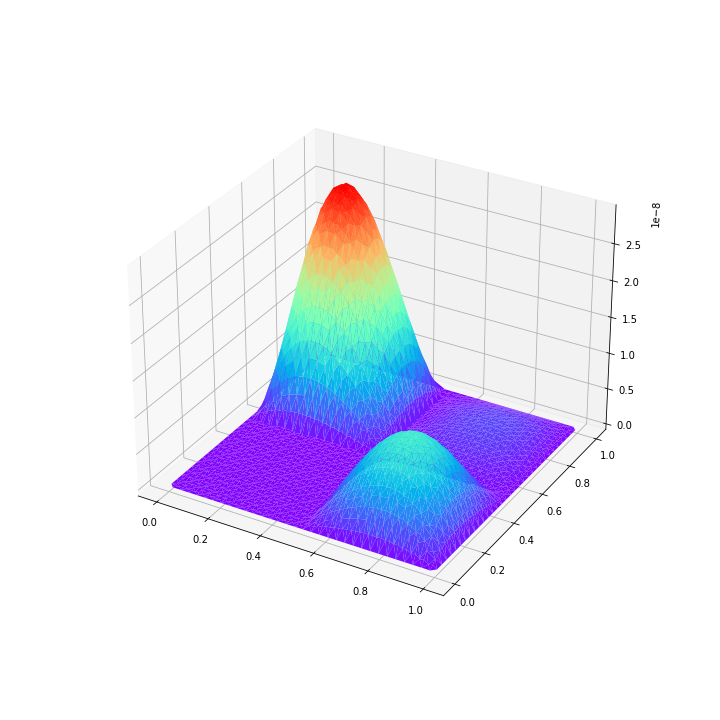
\includegraphics[height=4cm,width=4cm]{../image/ppt/uh_lam=[ 1].png}
	\hspace{0.9cm}
	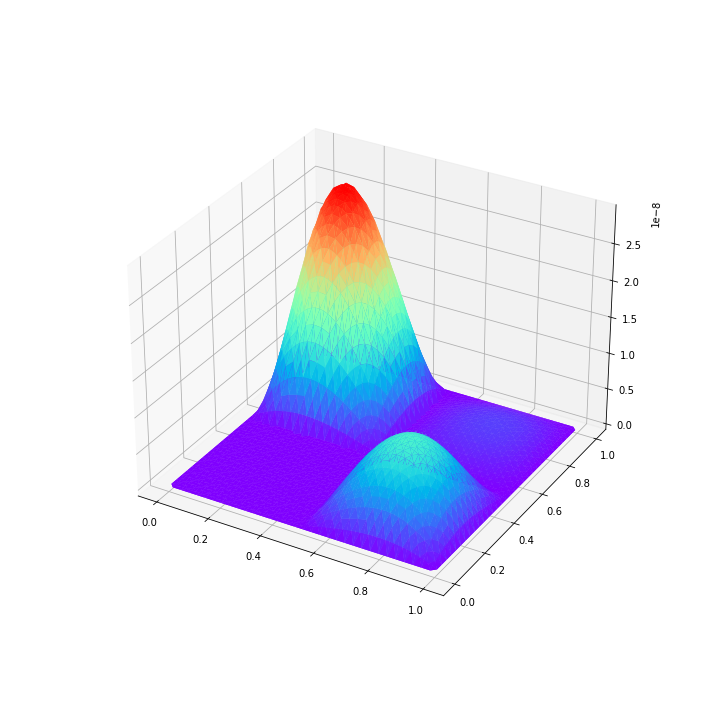
\includegraphics[height=4cm,width=4cm]{../image/ppt/u_lam=[ 1].png}
	\caption{数值解和精确解图像}
\end{figure}

\end{frame}

\begin{frame}
\item 当Lam$\acute{e}$ 常数 $\lambda = \mu= [7,3E2,2E3,10]$ 时误差如下
\vspace{0.6cm}
\begin{table}[h]
	\centering
	\scalebox{0.7}{
		\begin{tabular}{|c|c|c|c|c|} \toprule[1pt] \hline
			h &0.5 &0.25 &0.125 &0.0625 \\ \hline
			$|u-u_h|_{H^1(\Omega)}$ &1.599735E-2 &7.130099E-3 &3.516522E-3 &1.900428E-3  \\ \hline
			H1误差阶 &1.165839 &1.019772 &0.8878243 &0.918610 \\ \hline
			$|u-u_h|_{L^2(\Omega)}$ &3.999338E-3 &8.912623E-4 &2.197826E-4 &5.938839E-5  \\ \hline
			L2误差阶 &2.165839 &2.019772 &1.887824 &1.91861 \\ \hline	
			\bottomrule[1pt]
	\end{tabular}}
\end{table}

\begin{figure}
	\centering
	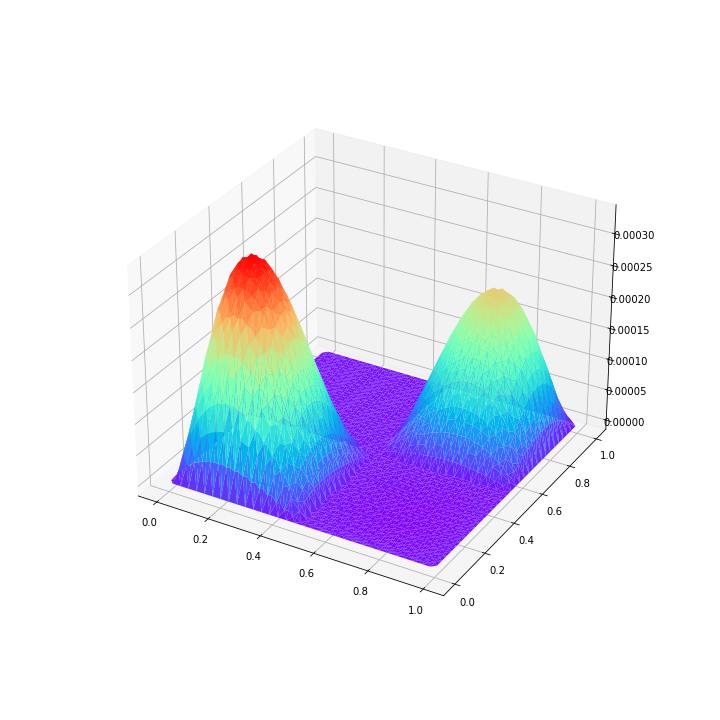
\includegraphics[height=4cm,width=4cm]{../image/ppt/uh_lam=[2].png}
	\hspace{0.9cm}
	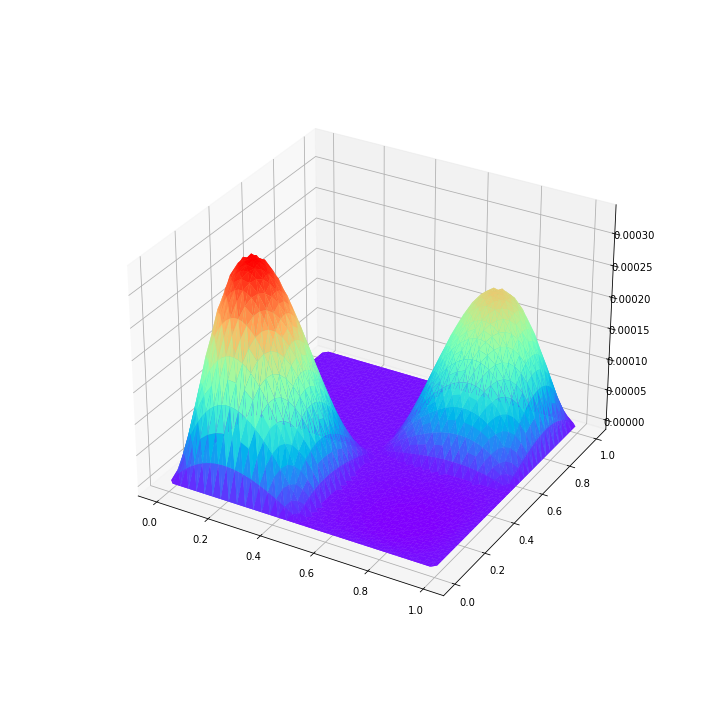
\includegraphics[height=4cm,width=4cm]{../image/ppt/u_lam=[2].png}
	\caption{数值解和精确解图像}
\end{figure}

\end{frame}

\begin{frame}
\item 当Lam$\acute{e}$ 常数 $\lambda = \mu= [7E8,5,1E4,3E6]$ 时误差如下
\vspace{0.6cm}
\begin{table}[h]
	\centering
	\scalebox{0.7}{
		\begin{tabular}{|c|c|c|c|c|} \toprule[1pt] \hline
			h &0.5 &0.25 &0.125 &0.0625 \\ \hline
			$|u-u_h|_{H^1(\Omega)}$ &3.015333E-3 &1.139928E-3 &6.718610E-4 &3.793589E-4  \\ \hline
			H1误差阶 &1.403373 &0.7627090 &0.8245995 &0.9054011 \\ \hline
			$|u-u_h|_{L^2(\Omega)}$ &7.538332E-4 &1.424911E-5 &4.199131E-5 &1.185496E-5  \\ \hline
			H1误差阶 &2.403373 &1.7627090 &1.824599 &1.905401 \\ \hline	
			\bottomrule[1pt]
	\end{tabular}}
\end{table}

\begin{figure}
	\centering
	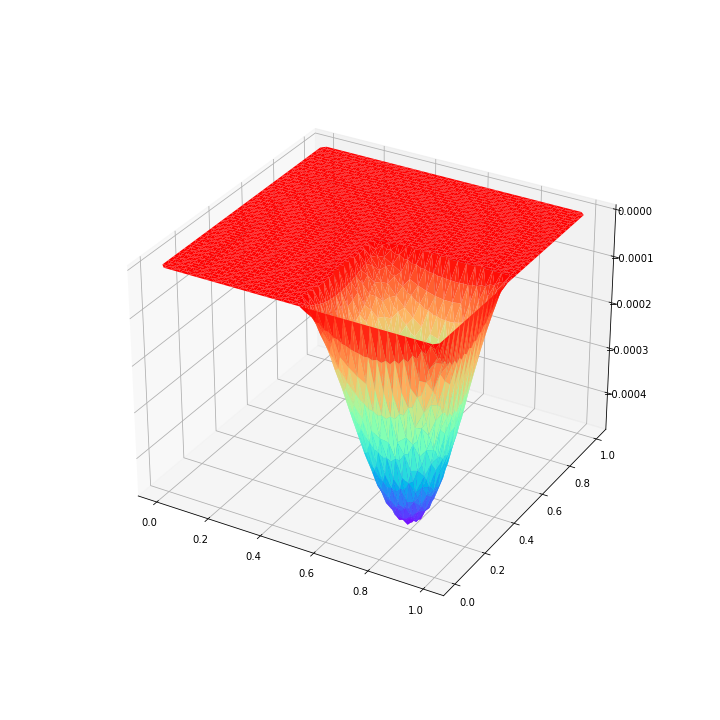
\includegraphics[height=4cm,width=4cm]{../image/ppt/uh_lam=[7.e+08 5.e+00 1.e+04 3.e+06].png}
	\hspace{0.9cm}
	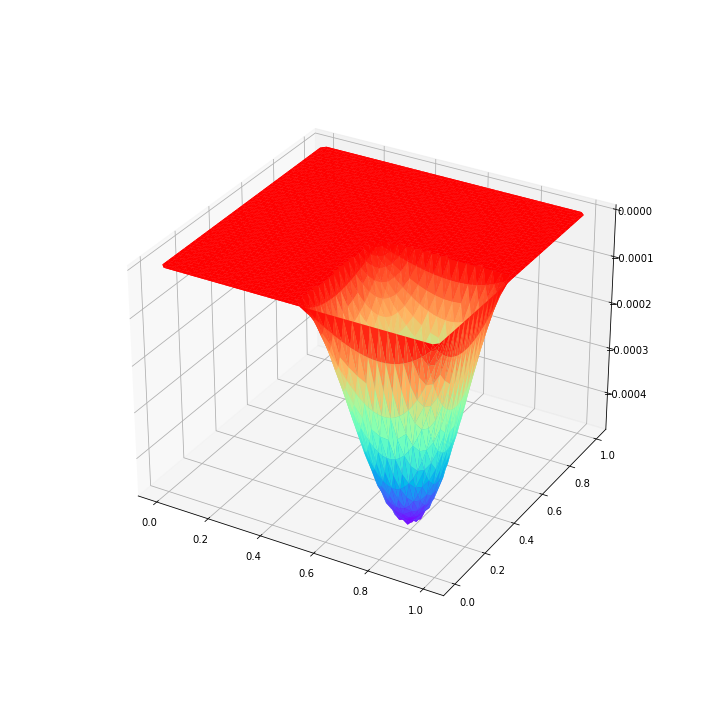
\includegraphics[height=4cm,width=4cm]{../image/ppt/u_lam=[7.e+08 5.e+00 1.e+04 3.e+06].png}
	\caption{数值解和精确解图像}
\end{figure}

\end{frame}
\end{enumerate} 

\section{总结}

\begin{frame}
	数值结果表明,当 Lam$\acute{e}$ 常数间断且相等时,C-R 元可以有效地解除闭锁现象,并且具有预期的收敛阶。
\end{frame}

\section{致谢}
\begin{frame}
	\begin{center}
		\huge 谢谢!
	\end{center}
\end{frame}


\end{document}
